\documentclass{article}
% template pour les futurs cr de math

\newcommand{\numprojet}{2} % Change pour mettre à jour le numéro de projet.

\usepackage{authblk} % Permet d'ajouter plusieurs auheur à un doc et ajouter des infos
\usepackage[french]{babel} % Ajoute le français comme langue du document
\usepackage[margin=3cm]{geometry} % Mise en page des marges
\usepackage[useregional]{datetime2} % Date de la machine
\usepackage{fancyhdr} % Mise en page
\usepackage{titling} % Permet d'utiliser le nom de l'autheur, le titre la date etc...
\usepackage{graphicx} % Pour les images
\graphicspath{ {./img/} } % Le chemin du dossier image
\usepackage{float} %Pour gérer les flotants

\usepackage{tkz-tab} % PAckage pour faire des figures avancée
% Comme un tableau de variation par exemple

\usepackage{amsmath,amssymb} % Pour faire des maths
\usepackage{datetime} %package for \today

\pagestyle{fancy} % Definir le header
%\fancyfoot[L]{\today}
%\fancyfoot[C]{MT05 - Projet n°\numprojet{}}
%\fancyfoot[C]{\thepage}
%\fancyhead[L]{Baptiste Toussaint}
%\fancyhead[R]{n° Étudiant: 47769}
\fancyhead[R]{Baptiste Toussaint, n° Étudiant: 47769}
\fancyfoot[R]{MT05 - Projet n°\numprojet}
\fancyfoot[C]{\thepage}

\title{MT05, Projet n°\numprojet{}: Transformation du plan}
\author{Baptiste Toussaint}
\affil{baptiste.toussaint@utt.fr}
\date{19 avril 2022}


\begin{document}

	\maketitle
	\thispagestyle{fancy}
	
	\tableofcontents
	
	\newpage	
	
	\section{Introduction et objectifs du projet}
	
	L'objectif de ce projet est d'évaluer les racines d'une fonction $f$, continue, par le biai de deux méthodes numériques: la méthode par dichotomie et la méthode de Newton.
	
	\section{Méthode par dichotomie}
	
	\subsection{Explication}
	
	\begin{itemize}
	\item Soit une fonction $f$, continue sur l'intervalle $[a,b]$
	\item $a<b$
	\item $f(a)f(b)<0$
	\end{itemize}
	
	D'après le théorème des valeurs intermédiaires, $f$ s'annule \underline{au moins} une fois sur $]a,b[$.
	Ce résultat se démontre facilement:\\
	Si $f(a)f(b)<0$, soit $f(a)<0$, soit $f(b)<0$
	mais pas les deux.
	Commme $f$ est continue (donc sans discontinuité), on pourra tracer sa courbe "sans lever le crayon". La courbe passera forcément par 0 si l'on veut relier les points $a$ et $b$.
	
	La méthode par dichotomie revient à prendre le point milieu de l'intervalle $[a,b]$: $c$, d'observer la position de $f(c)$ et la comparer avec 0. Si $f(c)<0$ alors la racine de $f$ se trouve dans l'intervalle $[a,c]$, sinon dans $[c,b]$, et ainsi de suite.
	
	De manière plus générale on va prendre $c=\frac{a+b}{2}$ et observer le signe de $f(a)f(c)$:
	\begin{itemize}
		\item Si $f(a)f(c) > 0$, alors $f(a)$ et $f(c)$ ont le même signe (différent de celui de $f(b)$, par définition),
		donc le changement de signe s'effectue dans l'intervalle $[c,b]$
		\item Si $f(a)f(c) < 0$, alors $f(a)$ et $f(c)$ n'ont pas le même signe,
		donc le changement de signe s'est effectué dans l'intervalle $[a,c]$
		\item La valeur de $f(c)$ est très proche de 0 ou égal à 0, alors on a trouvé la racine de $f$.
	\end{itemize}
	
	\subsection{Exemple: $f(x)=x^{3}-10x+2$}

	\subsubsection{Existance des racines}

	Tableau de variation de la fonction $f$.	

	\begin{center}
		\begin{tikzpicture}
   			\tkzTabInit{$x$ / 1 , $f'(x)$ / 1, $f(x)$ / 1.5}{$-\infty$, $-\frac{\sqrt{30}}{3}$, $\frac{\sqrt{30}}{3}$, $+\infty$}
   			\tkzTabLine{, +, z, -, z, +}
   			\tkzTabVar{-/ $-\infty$, +/ $\approx 14.172$, -/ $\approx -10.172$, +/ $+\infty$}
		\end{tikzpicture}
	\end{center}
	
	On peut définir trois intervalles sur $\mathbb{R}$: $]-\infty;-\frac{\sqrt{30}}{3}]$, $[-\frac{\sqrt{30}}{3};\frac{\sqrt{30}}{3}]$, $[\frac{\sqrt{30}}{3};+\infty[$. $f$ change de signe sur chacun de ces intervalles, et $f$ étant continue, on peut appliquer le théorème des valeurs intermédiaires, donc il existe une racine $t_{i}$ de $f$ sur chacun de ces intervalles tel que: $t_{1}<t_{2}<t_{3}$.
	
	\subsubsection{Détermination des racines par dichotomie}
	
	\begin{center}
		\begin{figure}[H]
			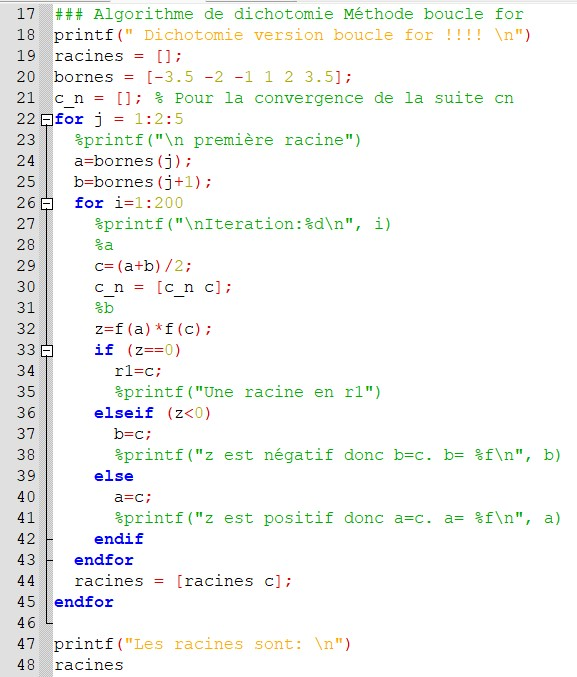
\includegraphics[scale=0.7]{./img/algo_racines_f_dicho_forloop.jpg}
		\end{figure}
	\end{center}
	
	Cette implémentation va rechercher les trois racines de f. La valeur de i (ligne 26) de la boucle for définira la précision de la recherche. Ici l'algorithme réalisera 200 itérations avant de rendre son résultat.
	
	Une autre solution est de passer par une boucle while, qui se basera sur une valeur d'erreur acceptable. Ici l'erreur sera de $10^{-8}$:
	
	\begin{center}
		\begin{figure}[H]
			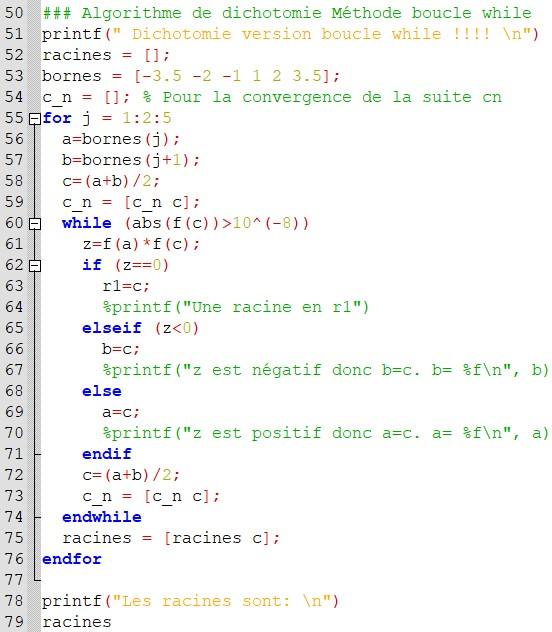
\includegraphics[scale=0.7]{./img/algo_racines_f_dicho_whileloop.jpg}
		\end{figure}
	\end{center}
	
	Dans les deux cas les algorithmes proposent des résultats égaux:

	\begin{center}
		\begin{figure}[H]
			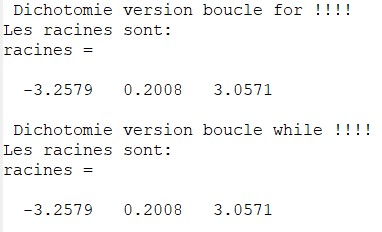
\includegraphics[scale=1]{./img/resultatrecherche.jpg}
		\end{figure}
	\end{center}
	
	Les racines de $f$ sont donc (approximativement)
	$R_{f}=\{-3.2579 ; 0.2008 ; 3.0571\}$
	
	\newpage	
	
	\subsection{Explication de la convergence}
	
	\subsubsection{Question 1}
	
	Soit $L_{0}$ la longeur de l'intervalle $[a_{0};\:b_{0}]$. On a alors:
	$L_{0}=\frac{b-a}{2}$.
	De même on a: $L_{1}=\frac{L_{0}}{2}$.
	
	Plus généralement on peut définir la récurence suivante:
	
	\begin{center}
		\begin{large}
			$L_{k+1}=\frac{L_{k}}{2}$
		\end{large}
	\end{center}
	
	Cette suite est une suite géométrique de raison $\frac{1}{2}$, donc on a:
	\begin{large}
		$$
		\left\{
			\begin{array}{ll}
				L_{0} = \frac{b+a}{2} \\ \\
				L_{k} = (\frac{b+a}{2}) \cdot (\frac{1}{2})^{k}
			\end{array}
		\right.
		$$
	\end{large}
	
	\subsubsection{Question 2}
	
	On a établit que le théorème des valeurs intermédiaires était applicable sur l'intervalle $]a; b[$ pour $f$, $f$ étant coninue sur cet intervalle (plus précisément, $f$ est un polynôme, donc de classe $C^{\infty}$ sur $\mathbb{R}$). Comme $f(a)f(b)<0$ et $f$ monotone sur $]a; b[$, il n'existe une unique racine $x^{*}$ sur $]a; b[$ (la monotonie garantit la bijectivité de la fonction et donc $f(x^{*})=0$ n'admet qu'une et une seule solution).
	
	A chaque itération de l'algorithme par dichotomie,
	l'intervalle de recherche est modifié en $]a';b'[$ comme suit:
	\begin{itemize}
		\item $a'=a$ et $b'=\frac{b+a}{2}$ ou
		\item $a'=\frac{b+a}{2}$ et $b'=b$
		\item $f(\frac{b+a}{2})=0$ , dans ce cas la racine est trouvée
	\end{itemize}
	Par définition à chaque itération, soit on trouve exactement la racine, soit elle se trouve dans l'intervalle $]a'; b'[$ nouvellement crée.
	
	Dans les deux cas $\frac{b+a}{2}$ appartient à $]a; b[$, donc $]a; \frac{b+a}{2}[$ comme $]\frac{b+a}{2}; b[$ sont des sous-intervalles de $]a';b'[$ et en possèdent les mêmes propriétés.\\
	
	On peut conclure qu'il n'existe une unique racine $x^{*}$ sur $]a'; b'[$.
	On pourra répéter ce principe jusqu'à $k$, les propriétés du théorème des valeurs intermédiaires resteront valide pour $]a_{k}; b_{k}[$. De ce fait on peut conclure qu'il existe une unique racine $x^{*}$ sur $]a_{k}; b_{k}[$, pour toutes valeurs de $k$.
	
	\subsubsection{Question 3}
	
	On a $c_{n}$ la suite qui correspond aux valeurs succesives des milieux de $[a; b]$.
	$c_{n}$ prend donc des valeurs réelles dans $\mathbb{R}$, aussi, on sait que $x^{*} \in [a; b]$ et $c_{n} \in [a; b]$. Par définition on a donc:
	
	\begin{center}
		\begin{large}
			$|c_{k}-x^{*}| < |b-a|$
		\end{large}
	\end{center}

	Une borne supérieure de la suite $|c_{k}-x^{*}|$ est donc $|b-a|$.
	
	On peut affiner cette borne. En effet on a:
	
	\begin{large}
		$$
		\left\{
			\begin{array}{ll}
				c_{0}= \frac{b_{0}-a_{0}}{2} \\ \\
				c_{k}= \frac{c_{k-1}+\frac{a_{k-1}}{b_{k-1}}}{2}
			\end{array}
		\right.
		$$
	\end{large}
	
	\newpage	
	
	A chaque itération de l'algorithme par dichotomie, on a $c_{k} \in [a_{k}; b_{k}]$ et
	$x^{*} \in [a_{k}; b_{k}]$. Donc par définition on a:
	
	\begin{center}
		\begin{large}
			$|c_{k}-x^{*}| < L_{k}$
		\end{large}
	\end{center}

	\subsection{Question 4}
	
	Donc $|c_{k}-x^{k}|$ est une suite majorée par $L_{k}$ et $|c_{k}-x^{k}| > 0$. Or $L_{k}$ converge vers 0. Donc $|c_{k}-x^{k}|$ converge vers 0 (théorème des gendarmes):
	
	\begin{center}
		\begin{large}
			$0 \le |c_{k}-x^{k}| < L_{k}$
		\end{large}
	\end{center}

	Donc:
	
	\begin{center}
		\begin{large}
			$|c_{k}-x^{*}| < L_{k}$\\
			$L_{k} < c_{k}-x^{*} < L_{k}$\\
			$x^{*}-L_{k} < c_{k} < L_{k}+x^{*}$\\
			$\lim_{k \to +\infty} (L_{k}) = 0$\\
			$\lim_{k \to +\infty} (x^{*}-L_{k} < c_{k} < L_{k}+x^{*}) = x^{*} < c_{k} < x^{*}$
		\end{large}
	\end{center}

	Donc $c_{k}$ converge vers $x^{*}$.

	\subsection{Question 5}
	
	On souhaite déterminer le nombre n minimal tel que: $|c_{n}-x^{*}|<\epsilon$. Si on prend $\epsilon = L_{n}$ Soit:	
	\begin{center}
		\begin{large}
			$L_{n} = \epsilon$\\
			$(\frac{b+a}{2}) \cdot (\frac{1}{2})^{n} = \epsilon$\\
			$(\frac{1}{2})^{n} = \frac{2 \epsilon}{b+a}$\\
			$2^{n} = \frac{b+a}{2 \epsilon}$\\
			$log_{2}(2^{n}) = log_{2}(\frac{b+a}{2 \epsilon})$\\
		\end{large}
	\end{center}
	
	Donc:
	
	\begin{center}
		\begin{large}
			$n = E(log_{2}(\frac{b+a}{2 \epsilon}))+1$
		\end{large}
	\end{center}

	Avec $E$ la partie entière.
	
	\subsection{Question 6}
	
	Si on prend $\epsilon = 10^{-10}$ on pour la  racine entre $2$ et $3.5$ a alors:
	
	\begin{center}
		\begin{large}
			$n=E(34.5412)+1$\\
			$n=35$
		\end{large}
	\end{center}

	\newpage

	\section{Méthode par l'algorithme de Newton}
	
	On va ici déterminer les facines de $f$ par la méthode
	de Newton.
	Cette méthode est très ancienne est était déjà utlisé par les grecs dans l'antiquité.
	On considère généralement que la méthode de Newton possède des meilleurs propriétées de convergences face à la dichotomie.
	
	\subsection{Racherche des racines}
	
	Dans cette partie nous allons travailler à la recherche de racine du polynôme $f(x)=x^{3}-10x+2$, dans
	$\mathbb{R}$ et $\mathbb{C}$.
	
	\subsubsection{Question 1}

	a)	
	
	Pour la fonction: $f(x)=x^{3}-10x+2$, nous pouvons appliquer l'algorithme de Newton suivant:
	
	\begin{large}
		$$
		\left\{
			\begin{array}{ll}
				x_{0} \\ \\
				x_{n+1}=x_{n}-\frac{x_{n}^{3}-10x_{n}+2}{3x_{n}^{2}-10}
			\end{array}
		\right.
		$$
	\end{large}

	b)	
	
	Pour rechercher les racines nous allons effectuer une recherche à partir d'un maillage de l'intervale $[-5; 5]$.
	L'intervale est découpé en 100 valeurs par pas de 0.1, et chacune de ces 100 valeurs sera un $x_{0}$ dont on étudiera la convergence. On obtient alors le code suivant: 
	
	\begin{center}
		\begin{figure}[H]
			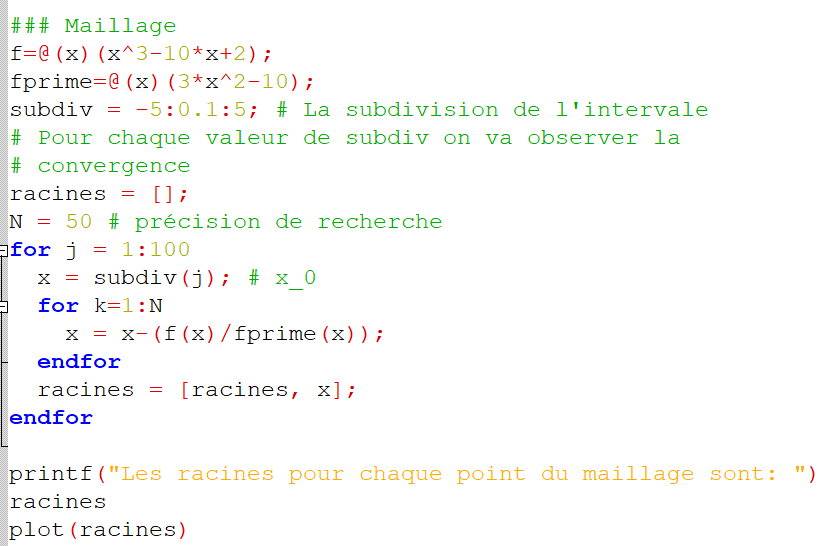
\includegraphics[scale=1]{./img/newton1.png}
		\end{figure}
	\end{center}
	
	On observe alors qu'il ressort 3 racines, identiques a celles trouvée par méthodes de dichotomie, et leurs répartition est comme suit:

	\begin{center}
		\begin{figure}[H]
			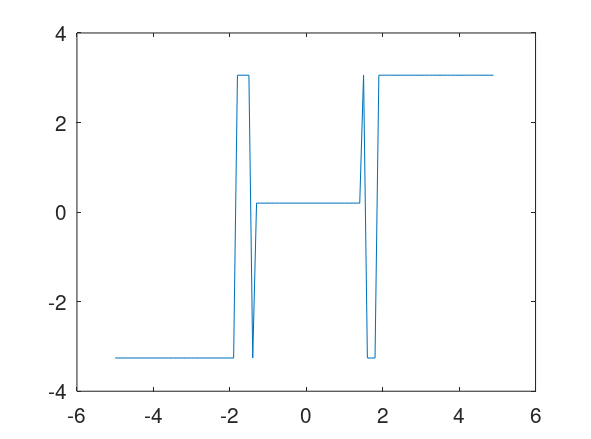
\includegraphics[scale=0.80]{./img/newton_conv_subdiv.png}
		\end{figure}
	\end{center}
	
	On observe que pour un $x_{0}$ proche de -5, la méthode converge vers -3.2579, pour $x_{0}$ proche de 0, la méthode converge vers 0.2008, et pour $x_{0}$ proche de 5, la méthode converge vers 3.0571. Il existe cependant des zones dégénéré, vers -1 et 1, qui correspondent aux extremum locaux de la fonction, là où sa dérivé est presque paralèlle aux abscisses.
	Dans ce cas la méthode de Newton va créer un $x_{n+1}$
	très loin de la racine recherchée et finira par converger sur l'une des deux racine latérales: -3.2579, et 3.0571.
	
	c)
	
	Par définition la méthode de Newton n'est pas définie pour $f'(x)=0$ (dénominateur nul). Les racines exactes de la dérivée sont: $-\sqrt{\frac{10}{3}}$, et $ \sqrt{\frac{10}{3}}$.
	
	Donc si $x_{n}$ est égale à l'une de ces racines, alors la méthode ne sera pas fonctionnelle.
	
	Cependant on peut ajouter que même sans commencer avec $x_{0}= \pm  \sqrt{\frac{10}{3}}$, il suffit prendre un $x_{0}$ dont la suite $x_{n}$ passera par $\pm \sqrt{\frac{10}{3}}$ pour que cette méthode ne fonctionne pas.
	
	\subsubsection{Question 2}
		
	On a la fonction $g(x)=\sqrt{|x|}$.
	Pour cette fonction la méthode ne pourra pas converger car la fonction n'admet pas de dérivée continue sur $\mathbb{R}$.
	
	Démonstration: 
	
	\begin{large}
	\begin{center}
		On pose $g(x)=\sqrt{h(x)}$ avec $h(x)=|x|$.\\
		Donc $g'(x)=\frac{1}{2\sqrt{h(x)}} \cdot h'(x)$,\\
		Donc: $g'(x)=\frac{1}{2\sqrt{|x|}} \cdot \pm 1$.
	
		$$g'(x)=\left\{
			\begin{array}{ll}
				\frac{1}{2\sqrt{x}} \mbox{, si } x > 0 \\ \\
				-\frac{1}{2\sqrt{-x}} \mbox{, si } x < 0				
			\end{array}\right.$$
	
	Or on a:

		$$
		\left\{
			\begin{array}{ll}
				lim_{0 \to 0^{+}}\frac{1}{2\sqrt{x}}=+\infty \\ \\
				lim_{0 \to 0^{-}}-\frac{1}{2\sqrt{-x}}=-\infty
			\end{array}
		\right.
		$$
	\end{center}
	\end{large}	

	Donc $g$ n'est pas de classe $C^{2}$ sur $\mathbb{R}$.
	
	\subsubsection{Question 3}
	
	On utilise aussi la méthode de Newton pour les fonctions holomorphes.
	
	Soit le polynôme sur $\mathbb{C}$:
	$f(z)=z^{3}-10z+2$. On peut déterminer les racines de ce polynôme par la méthode de Newton.
	
	On va créer un maillage de $\mathbb{C}$ en subdivisant l'axe des réel et des imaginaire en 100 valeurs entre -5 et 5.
	
	On obtiendra alors 10 000 valeurs de $x_{0}$ à tester pour la convergence.
	
	On obtiendra alors un vecteur de 10 000 valeurs complexes représentant les racines de la fonction.
	
	On retrouve alors les racines identiques à la fonction réelle correspondante:
	
	\begin{itemize}
		\item -3.2579 + 0i
		\item 0.2008 + 0i
		\item 3.0571 + 0i
	\end{itemize}

	\subsubsection{Question 4}
	
	On a $P(z)=z^{7}-2z^{3}+5$. Les racines de $P$ sont
	les $z_{*}$ tel que:
	$P(z_{*})=z_{*}^{7}-2z_{*}^{3}+5=0$
	
	On a donc:
	
	\begin{large}
	\begin{center}
		$z_{*}^{7}-2z_{*}^{3}+5=0$\\
		$z_{*}^{7}=2z_{*}^{3}-5$\\
		$|z_{*}^{7}|=|2z_{*}^{3}-5|$\\
		$|z_{*}^{7}| \le 2|z_{*}|^{3}+5$
	\end{center}
	\end{large}	
	
	On pose $X=|z_{*}|$ ce qui donne:
	
	\begin{large}
	\begin{center}
			$X^{7} \le 2X^{3}-5$ 
	\end{center}	
	\end{large}
	
	Si on prend $X=|z_{*}|=2$ on a alors une incohérence: 
	
	\begin{large}
	\begin{center}
			$2^{7} \le 2^{4}-5$
			$128 \le 11$
	\end{center}	
	\end{large}
	
	Donc on peut affirmer que $|z_{*}|$, les racines de $P$ sont tel que: $|z_{*}| \in [0; 2[$.
	
	\subsubsection{Question 5}
	
	Pour retrouver numériquement ces racines ont utilise le code suivant:
	
	\begin{center}
		\begin{figure}[H]
			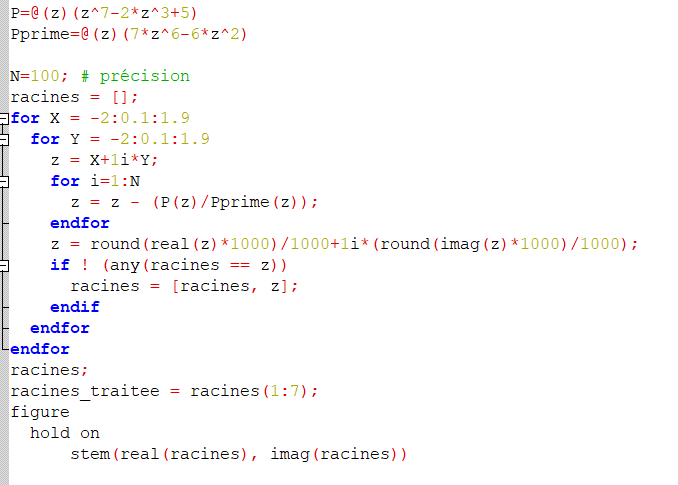
\includegraphics[scale=1]{./img/algo_new_deg_7.png}
		\end{figure}
	\end{center}
	
	Cet algorithme nous donne 9 racines, dont deux qui semblent être des racines dégénérées due à des valeurs de $z_{0}$ pour lesquelles l'algorithme ne fonctionne pas.
	
	\begin{center}
		\begin{figure}[H]
			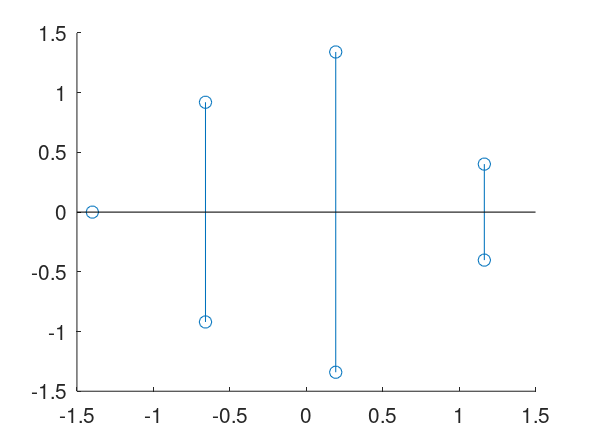
\includegraphics[scale=0.7]{./img/deg7newtonracines.png}
		\end{figure}
	\end{center}

	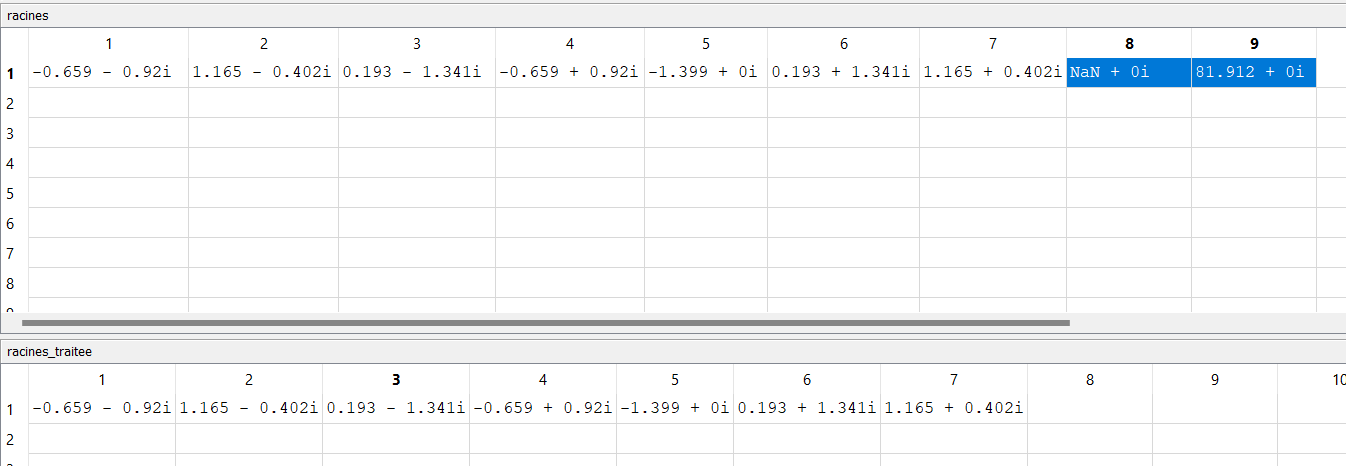
\includegraphics[scale=0.6]{./img/racines_new_deg7.png}
	
	Les racines sont donc environ égales à:
	
	\begin{itemize}
		\item 1: $-0.659-0.92i$
		\item 2: $1.165-0.402i$
		\item 3: $0.193-1.341i$
		\item 4: $-0.659+0.92i$
		\item 5: $-1.399+0i$
		\item 6: $0.193+1.341i$
		\item 7: $1.165+0.402i$
	\end{itemize}
	
	\newpage
	
	\subsection{Convergence de l'algorithme de Newton}
	
	Pour évaluer les performances de convergences de l'algorithme de Newton il faut remplir plusieurs prérequis :
	\begin{itemize}
		\item $f$ holomorphe, ou à valeurs réelles deux fois continûment dérivable
		\item $x^{*}$ est racine de f
		\item $f(x^{*})=0$
		\item $f'(x^{*}) \neq 0$
	\end{itemize}
	
	Pour rappel, analytiquement, les fonctions holomorphes correspondent à des fonctions ne faisant pas intervenir $\bar{z}$. Géométriquement, les fonctions holomorphes conservent les angles.\\
	
	On souhaite prouver qu'avec l'algorithme de Newton, il existe un voisinage V de $x^{*}$ tel que $x_{0} \in V$ et $x_{n+1}=x_{n}-\frac{f(x_{n})}{f'(x_{n})}$ converge vers $x_{*}$.\\
	
	\subsubsection{Question 1}
	
	On a $x_{n+1}=g(x_{n})$,
	avec $g(z)=(id-\frac{f}{f'})(z)$,
	donc $g(z)=z-\frac{f(z)}{f'(z)}$.
	
	\subsubsection{Question 2}
	
	$g(x^{*})=x^{*}-\frac{f(x^{*})}{f'(x^{*})}$.
	Donc on a $g(x^{*})=x^{*}$, car $f(x^{*})=0$.
	Les racines de $f$ sont donc les points fixes de la transformation $g$.

	\subsubsection{Question 3}
	
	$g'(z)=1-\frac{(f'(z))^{2}-f''(z)f(z)}{(f'(z))^{2}}$, donc
	$g'(x^{*})=1-\frac{(f'(x^{*}))^{2}-f''(x^{*})f(x^{*})}{(f'(x^{*}))^{2}}$
	$=1-\frac{(f'(x^{*}))^{2}}{(f'(x^{*}))^{2}}=1-1=0$.
	
	\subsubsection{Question 4}
	
	On a établit que $g(x_{n})=x_{n+1}$ est convergente vers $x^{*}$.\\
	
	On peut se retourner vers la définiton de la convergence:\\
	
	\begin{center}
	\begin{large}
		$(\exists \epsilon>0)(\exists N \in \Omega)$
		$(\forall n \in \Omega)(\exists l \in \Omega)$\\
		$n \geq N \Rightarrow |g(z)-l| < \epsilon$		\end{large}
	\end{center}
	
	Or ici on a:\\
	
	\begin{center}
		\begin{large}
			$lim_{z \to x^{*}}(g'(z))=$
			$lim_{z \to x^{*}}(1-\frac{(f'(z))^{2}-f''(z)f(z)}{(f'(z))^{2}})$\\
			$=0$.
		\end{large}
	\end{center}
	
	Donc on peut dire que $g'(z)$ converge vers $x^{*}$, donc: 
	
	\begin{center}
	\begin{large}
		$(\exists \epsilon>0)(\exists Z \in \Omega)$
		$(\forall z \in \Omega)$\\
		$z \geq Z \Rightarrow |g'(z)-0| < \epsilon
$\\
	$z \geq Z \Rightarrow |g'(z)| < \epsilon < 1
$
	\end{large}
	\end{center}
	
	\subsubsection{Question 5}
	
	On a:
	
	\begin{center}
		\begin{large}
			$g(x)=x-\frac{f(x)}{f'(x)}$\\
			$g(y)=y-\frac{f(y)}{f'(y)}$\\
			$g(x)-g(y)=x-\frac{f(x)}{f'(x)}-y+\frac{f(y)}{f'(y)}$
			$=x-y+\frac{f(y)}{f'(y)}-\frac{f(x)}{f'(x)}$\\
			$|g(x)-g(y)| = |x-y+\frac{f(y)}{f'(y)}-\frac{f(x)}{f'(x)}|$\\
			$|g(x)-g(y)| \le |x-y|+|\frac{f(y)}{f'(y)}-\frac{f(x)}{f'(x)}|$\\
			$|g(x)-g(y)| \le \epsilon|x-y|$
		\end{large}
	\end{center}		
	
	Avec: $\epsilon = 1 + \frac{|\frac{f(y)}{f'(y)}-\frac{f(x)}{f'(x)}|}{|x-y|}$
	
	\subsubsection{Question 6}
	
	\begin{center}
		\begin{large}
			$|g(z)-x^{*}| = |g(z)-g(x^{*})|$\\
			$|g(z)-x^{*}| \le \epsilon|z-x^{*}|$\\
			$|g(z)-x^{*}| \le |z-x^{*}|+|\frac{f(x^{*})}{f'(x^{*})}-\frac{f(z)}{f'(z)}|$\\
			$|g(z)-x^{*}| \le |z-x^{*}|+|-\frac{f(z)}{f'(z)}|$\\
		\end{large}
	\end{center}
	
	On peut poser $\alpha = |z-x^{*}|+|\frac{f(z)}{f'(z)}|$, et on a alors:
	
	\begin{center}
		\begin{large}
			$|g(z)-x^{*}| \le \alpha$
		\end{large}
	\end{center}
	
	\subsubsection{Question 7}
	
	On prend $x_{0} \in V$, or on a établit que:
	\begin{itemize}
		\item $x_{n+1}=g(x_{n})$
		\item L'image de $z$ par $g$ appartient à $V$
	\end{itemize}
	
	Donc Par définiton, si $x_{n} \in V$ alors $x_{n+1} \in V$.\\
	
	La propriétée est initialisé pour $x_{0}$, et est héréditaire, donc par récurence on a $\forall n \in \mathbb{N}, x_{n} \in V$.
	
	\subsubsection{Question 8}
	
	On a:
	
	\begin{center}
		\begin{large}
			$\forall x \in V, \forall y \in V,$
			$|g(x)-g(y)| < \epsilon|x-y|$	
		\end{large}
	\end{center}

	Donc on a:
	
	\begin{center}
		\begin{large}
			$|g(x_{n+1})-g(x*)| < \epsilon|x_{n+1}-x^{*}|$\\
			$\epsilon|x_{n+1}-x^{*}| = \epsilon|g(x_{n})-g(x^{*})|$\\
			$\epsilon|g(x_{n})-g(x^{*})| < \epsilon^{2}|x_{n}-x^{*}|$\\
			$|g(x_{n+1})-g(x^{*})| < \epsilon^{2}|x_{n}-x^{*}|$
		\end{large}
	\end{center}

	\newpage	
	
	Donc on a:
	
	\begin{center}
		\begin{large}
			$|g(x_{n})-g(x*)| < \epsilon^{1}|x_{n}-x^{*}|$\\
			$\epsilon|x_{n}-x^{*}| = \epsilon^{1}|g(x_{n-1})-g(x^{*})|$\\
			$\epsilon|g(x_{n-1})-g(x^{*})| < \epsilon^{2}|x_{n-1}-x^{*}|$\\
			$|g(x_{n})-g(x^{*})| < \epsilon^{2}|x_{n-1}-x^{*}|$\\
			...\\
			$|g(x_{n})-g(x^{*})| < \epsilon^{n}|x_{0}-x^{*}|$\\
		\end{large}
	\end{center}
	
	\subsubsection{Question 9}
	
	L'algorithme de Newton va créer une suite de $x_{n}$ à partir d'une valeur $x_{0}$. Les valeurs de $x_{n+1}$ sont
	donné par la relation $g(x_{n})=x_{n+1}$.\\
	
	En faisant tourner l'algorithme pour n valeurs. On obtiendra alors une valeur de $x_{n}$ qui devra être le plus proche de $x^{*}$ la racine de la fonction $f$.\\
	
	On a montré que:
	
	\begin{center}
		\begin{large}
			$|g(x_{n})-g(x^{*})| < \epsilon^{n}|x_{0}-x^{*}|$\\
			$|g(x_{n})-x^{*}| < \epsilon^{n}|x_{0}-x^{*}|$
		\end{large}
	\end{center}
	
	Donc pour un $x_{0}$ donné, après n étapes de l'algorithme, l'écart relatif entre $x_{0}$ et la valeur atteinte $g(x_{n})=x_{n+1}$ est bornée par l'écart entre $x_{0}$ et $x^{*}$, multiplié par un facteur $\epsilon$ à la puissance n.
	Et ce, pour tout n appartenant à $\mathbb{N}$.\\
	
	On a donc montré que la suite des $x_{n}$ converge vers la valeur $x^{*}$, racine de $f$. On peut conclure que l'algorithme de Newton converge. On peut préciser que cet algorithme converge avec une vitesse remarquable en $\epsilon^{n}$, ce qui est bien meilleur que la méthode par dichotomies.
	
\end{document}